% !TEX encoding = UTF-8 Unicode
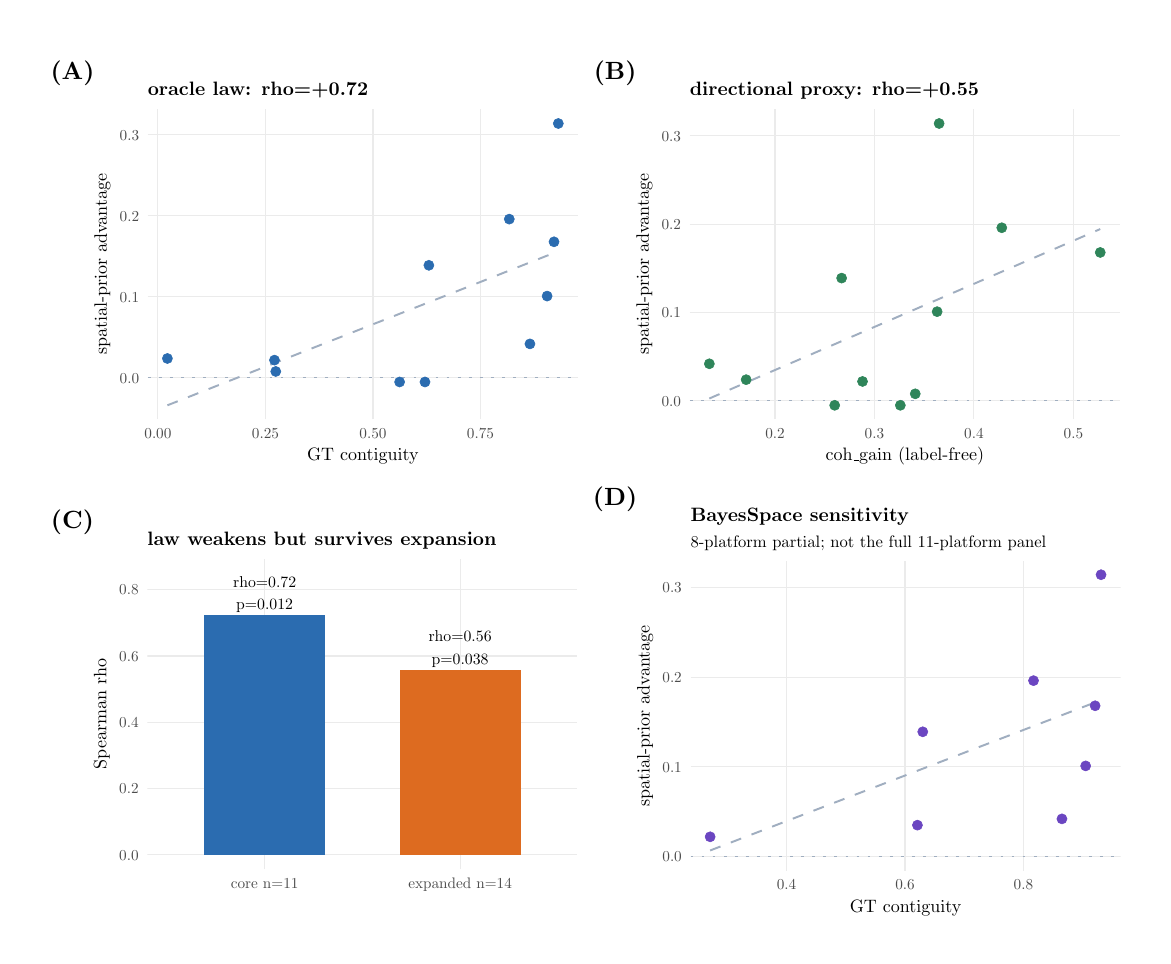
\begin{tikzpicture}[x=1pt,y=1pt]
\definecolor{fillColor}{RGB}{255,255,255}
\path[use as bounding box,fill=fillColor,fill opacity=0.00] (0,0) rectangle (403.13,328.16);
\begin{scope}
\path[clip] (  0.00,  0.00) rectangle (403.13,328.16);
\definecolor{drawColor}{RGB}{255,255,255}
\definecolor{fillColor}{RGB}{255,255,255}

\path[draw=drawColor,line width= 0.6pt,line join=round,line cap=round,fill=fillColor] (  0.00,  0.00) rectangle (403.13,328.16);
\end{scope}
\begin{scope}
\path[clip] (  5.50,164.08) rectangle (201.56,322.66);
\definecolor{drawColor}{RGB}{255,255,255}
\definecolor{fillColor}{RGB}{255,255,255}

\path[draw=drawColor,line width= 0.6pt,line join=round,line cap=round,fill=fillColor] (  5.50,164.08) rectangle (201.56,322.66);
\end{scope}
\begin{scope}
\path[clip] (201.56,164.08) rectangle (397.63,322.66);
\definecolor{drawColor}{RGB}{255,255,255}
\definecolor{fillColor}{RGB}{255,255,255}

\path[draw=drawColor,line width= 0.6pt,line join=round,line cap=round,fill=fillColor] (201.56,164.08) rectangle (397.63,322.66);
\end{scope}
\begin{scope}
\path[clip] (  4.26,167.04) rectangle (202.80,319.70);
\definecolor{fillColor}{RGB}{255,255,255}

\path[fill=fillColor] (  4.26,167.04) rectangle (202.80,319.70);
\end{scope}
\begin{scope}
\path[clip] ( 43.42,186.61) rectangle (198.80,298.63);
\definecolor{drawColor}{gray}{0.92}

\path[draw=drawColor,line width= 0.4pt,line join=round] ( 43.42,201.59) --
	(198.80,201.59);

\path[draw=drawColor,line width= 0.4pt,line join=round] ( 43.42,230.87) --
	(198.80,230.87);

\path[draw=drawColor,line width= 0.4pt,line join=round] ( 43.42,260.15) --
	(198.80,260.15);

\path[draw=drawColor,line width= 0.4pt,line join=round] ( 43.42,289.43) --
	(198.80,289.43);

\path[draw=drawColor,line width= 0.4pt,line join=round] ( 47.07,186.61) --
	( 47.07,298.63);

\path[draw=drawColor,line width= 0.4pt,line join=round] ( 85.92,186.61) --
	( 85.92,298.63);

\path[draw=drawColor,line width= 0.4pt,line join=round] (124.77,186.61) --
	(124.77,298.63);

\path[draw=drawColor,line width= 0.4pt,line join=round] (163.61,186.61) --
	(163.61,298.63);
\definecolor{drawColor}{RGB}{160,174,192}

\path[draw=drawColor,line width= 0.4pt,dash pattern=on 1pt off 3pt ,line join=round] ( 43.42,201.59) -- (198.80,201.59);

\path[draw=drawColor,line width= 0.7pt,dash pattern=on 4pt off 4pt ,line join=round] ( 50.49,191.70) --
	( 52.27,192.40) --
	( 54.06,193.11) --
	( 55.85,193.81) --
	( 57.64,194.52) --
	( 59.43,195.22) --
	( 61.21,195.93) --
	( 63.00,196.63) --
	( 64.79,197.34) --
	( 66.58,198.04) --
	( 68.37,198.75) --
	( 70.15,199.45) --
	( 71.94,200.16) --
	( 73.73,200.86) --
	( 75.52,201.56) --
	( 77.31,202.27) --
	( 79.09,202.97) --
	( 80.88,203.68) --
	( 82.67,204.38) --
	( 84.46,205.09) --
	( 86.25,205.79) --
	( 88.04,206.50) --
	( 89.82,207.20) --
	( 91.61,207.91) --
	( 93.40,208.61) --
	( 95.19,209.32) --
	( 96.98,210.02) --
	( 98.76,210.73) --
	(100.55,211.43) --
	(102.34,212.13) --
	(104.13,212.84) --
	(105.92,213.54) --
	(107.70,214.25) --
	(109.49,214.95) --
	(111.28,215.66) --
	(113.07,216.36) --
	(114.86,217.07) --
	(116.64,217.77) --
	(118.43,218.48) --
	(120.22,219.18) --
	(122.01,219.89) --
	(123.80,220.59) --
	(125.58,221.30) --
	(127.37,222.00) --
	(129.16,222.71) --
	(130.95,223.41) --
	(132.74,224.11) --
	(134.52,224.82) --
	(136.31,225.52) --
	(138.10,226.23) --
	(139.89,226.93) --
	(141.68,227.64) --
	(143.46,228.34) --
	(145.25,229.05) --
	(147.04,229.75) --
	(148.83,230.46) --
	(150.62,231.16) --
	(152.40,231.87) --
	(154.19,232.57) --
	(155.98,233.28) --
	(157.77,233.98) --
	(159.56,234.69) --
	(161.34,235.39) --
	(163.13,236.09) --
	(164.92,236.80) --
	(166.71,237.50) --
	(168.50,238.21) --
	(170.28,238.91) --
	(172.07,239.62) --
	(173.86,240.32) --
	(175.65,241.03) --
	(177.44,241.73) --
	(179.23,242.44) --
	(181.01,243.14) --
	(182.80,243.85) --
	(184.59,244.55) --
	(186.38,245.26) --
	(188.17,245.96) --
	(189.95,246.66) --
	(191.74,247.37);
\definecolor{drawColor}{RGB}{43,108,176}
\definecolor{fillColor}{RGB}{43,108,176}

\path[draw=drawColor,line width= 0.2pt,line join=round,line cap=round,fill=fillColor] (187.70,231.17) circle (  1.83);

\path[draw=drawColor,line width= 0.2pt,line join=round,line cap=round,fill=fillColor] (143.57,200.13) circle (  1.83);

\path[draw=drawColor,line width= 0.2pt,line join=round,line cap=round,fill=fillColor] (191.74,293.53) circle (  1.83);

\path[draw=drawColor,line width= 0.2pt,line join=round,line cap=round,fill=fillColor] (190.19,250.78) circle (  1.83);

\path[draw=drawColor,line width= 0.2pt,line join=round,line cap=round,fill=fillColor] (174.03,258.98) circle (  1.83);

\path[draw=drawColor,line width= 0.2pt,line join=round,line cap=round,fill=fillColor] ( 89.18,208.03) circle (  1.83);

\path[draw=drawColor,line width= 0.2pt,line join=round,line cap=round,fill=fillColor] (181.49,213.89) circle (  1.83);

\path[draw=drawColor,line width= 0.2pt,line join=round,line cap=round,fill=fillColor] (144.97,242.29) circle (  1.83);

\path[draw=drawColor,line width= 0.2pt,line join=round,line cap=round,fill=fillColor] (134.40,200.13) circle (  1.83);

\path[draw=drawColor,line width= 0.2pt,line join=round,line cap=round,fill=fillColor] ( 89.65,203.93) circle (  1.83);

\path[draw=drawColor,line width= 0.2pt,line join=round,line cap=round,fill=fillColor] ( 50.49,208.62) circle (  1.83);
\end{scope}
\begin{scope}
\path[clip] (  0.00,  0.00) rectangle (403.13,328.16);
\definecolor{drawColor}{gray}{0.30}

\node[text=drawColor,anchor=base east,inner sep=0pt, outer sep=0pt, scale=  0.55] at ( 40.27,199.70) {0.0};

\node[text=drawColor,anchor=base east,inner sep=0pt, outer sep=0pt, scale=  0.55] at ( 40.27,228.98) {0.1};

\node[text=drawColor,anchor=base east,inner sep=0pt, outer sep=0pt, scale=  0.55] at ( 40.27,258.26) {0.2};

\node[text=drawColor,anchor=base east,inner sep=0pt, outer sep=0pt, scale=  0.55] at ( 40.27,287.54) {0.3};
\end{scope}
\begin{scope}
\path[clip] (  0.00,  0.00) rectangle (403.13,328.16);
\definecolor{drawColor}{gray}{0.30}

\node[text=drawColor,anchor=base,inner sep=0pt, outer sep=0pt, scale=  0.55] at ( 47.07,179.67) {0.00};

\node[text=drawColor,anchor=base,inner sep=0pt, outer sep=0pt, scale=  0.55] at ( 85.92,179.67) {0.25};

\node[text=drawColor,anchor=base,inner sep=0pt, outer sep=0pt, scale=  0.55] at (124.77,179.67) {0.50};

\node[text=drawColor,anchor=base,inner sep=0pt, outer sep=0pt, scale=  0.55] at (163.61,179.67) {0.75};
\end{scope}
\begin{scope}
\path[clip] (  0.00,  0.00) rectangle (403.13,328.16);
\definecolor{drawColor}{RGB}{0,0,0}

\node[text=drawColor,anchor=base,inner sep=0pt, outer sep=0pt, scale=  0.65] at (121.11,171.58) {GT contiguity};
\end{scope}
\begin{scope}
\path[clip] (  0.00,  0.00) rectangle (403.13,328.16);
\definecolor{drawColor}{RGB}{0,0,0}

\node[text=drawColor,rotate= 90.00,anchor=base,inner sep=0pt, outer sep=0pt, scale=  0.65] at ( 28.61,242.62) {spatial-prior advantage};
\end{scope}
\begin{scope}
\path[clip] (  0.00,  0.00) rectangle (403.13,328.16);
\definecolor{drawColor}{RGB}{0,0,0}

\node[text=drawColor,anchor=base west,inner sep=0pt, outer sep=0pt, scale=  0.70] at ( 43.42,303.67) {\bfseries oracle law: rho=+0.72};
\end{scope}
\begin{scope}
\path[clip] (  0.00,  0.00) rectangle (403.13,328.16);
\definecolor{drawColor}{RGB}{0,0,0}

\node[text=drawColor,anchor=base,inner sep=0pt, outer sep=0pt, scale=  0.90] at ( 16.19,309.50) {\bfseries (A)};
\end{scope}
\begin{scope}
\path[clip] (200.55,167.04) rectangle (398.64,319.70);
\definecolor{fillColor}{RGB}{255,255,255}

\path[fill=fillColor] (200.55,167.04) rectangle (398.64,319.70);
\end{scope}
\begin{scope}
\path[clip] (239.26,186.61) rectangle (394.64,298.63);
\definecolor{drawColor}{gray}{0.92}

\path[draw=drawColor,line width= 0.4pt,line join=round] (239.26,193.29) --
	(394.64,193.29);

\path[draw=drawColor,line width= 0.4pt,line join=round] (239.26,225.22) --
	(394.64,225.22);

\path[draw=drawColor,line width= 0.4pt,line join=round] (239.26,257.14) --
	(394.64,257.14);

\path[draw=drawColor,line width= 0.4pt,line join=round] (239.26,289.06) --
	(394.64,289.06);

\path[draw=drawColor,line width= 0.4pt,line join=round] (270.04,186.61) --
	(270.04,298.63);

\path[draw=drawColor,line width= 0.4pt,line join=round] (305.98,186.61) --
	(305.98,298.63);

\path[draw=drawColor,line width= 0.4pt,line join=round] (341.93,186.61) --
	(341.93,298.63);

\path[draw=drawColor,line width= 0.4pt,line join=round] (377.87,186.61) --
	(377.87,298.63);
\definecolor{drawColor}{RGB}{160,174,192}

\path[draw=drawColor,line width= 0.4pt,dash pattern=on 1pt off 3pt ,line join=round] (239.26,193.29) -- (394.64,193.29);

\path[draw=drawColor,line width= 0.7pt,dash pattern=on 4pt off 4pt ,line join=round] (246.32,194.16) --
	(248.11,194.94) --
	(249.89,195.71) --
	(251.68,196.49) --
	(253.47,197.26) --
	(255.26,198.04) --
	(257.05,198.81) --
	(258.83,199.59) --
	(260.62,200.36) --
	(262.41,201.14) --
	(264.20,201.91) --
	(265.99,202.69) --
	(267.77,203.46) --
	(269.56,204.24) --
	(271.35,205.01) --
	(273.14,205.79) --
	(274.93,206.56) --
	(276.71,207.34) --
	(278.50,208.11) --
	(280.29,208.89) --
	(282.08,209.66) --
	(283.87,210.44) --
	(285.65,211.21) --
	(287.44,211.99) --
	(289.23,212.76) --
	(291.02,213.54) --
	(292.81,214.31) --
	(294.59,215.09) --
	(296.38,215.86) --
	(298.17,216.64) --
	(299.96,217.41) --
	(301.75,218.19) --
	(303.54,218.96) --
	(305.32,219.74) --
	(307.11,220.51) --
	(308.90,221.29) --
	(310.69,222.06) --
	(312.48,222.84) --
	(314.26,223.61) --
	(316.05,224.39) --
	(317.84,225.16) --
	(319.63,225.94) --
	(321.42,226.71) --
	(323.20,227.49) --
	(324.99,228.26) --
	(326.78,229.04) --
	(328.57,229.81) --
	(330.36,230.59) --
	(332.14,231.36) --
	(333.93,232.14) --
	(335.72,232.91) --
	(337.51,233.69) --
	(339.30,234.46) --
	(341.08,235.24) --
	(342.87,236.01) --
	(344.66,236.79) --
	(346.45,237.56) --
	(348.24,238.34) --
	(350.02,239.11) --
	(351.81,239.89) --
	(353.60,240.66) --
	(355.39,241.44) --
	(357.18,242.21) --
	(358.96,242.99) --
	(360.75,243.76) --
	(362.54,244.54) --
	(364.33,245.31) --
	(366.12,246.09) --
	(367.90,246.86) --
	(369.69,247.64) --
	(371.48,248.41) --
	(373.27,249.19) --
	(375.06,249.96) --
	(376.84,250.74) --
	(378.63,251.51) --
	(380.42,252.29) --
	(382.21,253.06) --
	(384.00,253.84) --
	(385.78,254.61) --
	(387.57,255.39);
\definecolor{drawColor}{RGB}{47,133,90}
\definecolor{fillColor}{RGB}{47,133,90}

\path[draw=drawColor,line width= 0.2pt,line join=round,line cap=round,fill=fillColor] (328.63,225.54) circle (  1.83);

\path[draw=drawColor,line width= 0.2pt,line join=round,line cap=round,fill=fillColor] (315.33,191.70) circle (  1.83);

\path[draw=drawColor,line width= 0.2pt,line join=round,line cap=round,fill=fillColor] (329.35,293.53) circle (  1.83);

\path[draw=drawColor,line width= 0.2pt,line join=round,line cap=round,fill=fillColor] (387.57,246.93) circle (  1.83);

\path[draw=drawColor,line width= 0.2pt,line join=round,line cap=round,fill=fillColor] (351.99,255.86) circle (  1.83);

\path[draw=drawColor,line width= 0.2pt,line join=round,line cap=round,fill=fillColor] (301.67,200.32) circle (  1.83);

\path[draw=drawColor,line width= 0.2pt,line join=round,line cap=round,fill=fillColor] (246.32,206.70) circle (  1.83);

\path[draw=drawColor,line width= 0.2pt,line join=round,line cap=round,fill=fillColor] (294.12,237.67) circle (  1.83);

\path[draw=drawColor,line width= 0.2pt,line join=round,line cap=round,fill=fillColor] (291.61,191.70) circle (  1.83);

\path[draw=drawColor,line width= 0.2pt,line join=round,line cap=round,fill=fillColor] (320.72,195.85) circle (  1.83);

\path[draw=drawColor,line width= 0.2pt,line join=round,line cap=round,fill=fillColor] (259.62,200.96) circle (  1.83);
\end{scope}
\begin{scope}
\path[clip] (  0.00,  0.00) rectangle (403.13,328.16);
\definecolor{drawColor}{gray}{0.30}

\node[text=drawColor,anchor=base east,inner sep=0pt, outer sep=0pt, scale=  0.55] at (236.11,191.40) {0.0};

\node[text=drawColor,anchor=base east,inner sep=0pt, outer sep=0pt, scale=  0.55] at (236.11,223.32) {0.1};

\node[text=drawColor,anchor=base east,inner sep=0pt, outer sep=0pt, scale=  0.55] at (236.11,255.25) {0.2};

\node[text=drawColor,anchor=base east,inner sep=0pt, outer sep=0pt, scale=  0.55] at (236.11,287.17) {0.3};
\end{scope}
\begin{scope}
\path[clip] (  0.00,  0.00) rectangle (403.13,328.16);
\definecolor{drawColor}{gray}{0.30}

\node[text=drawColor,anchor=base,inner sep=0pt, outer sep=0pt, scale=  0.55] at (270.04,179.67) {0.2};

\node[text=drawColor,anchor=base,inner sep=0pt, outer sep=0pt, scale=  0.55] at (305.98,179.67) {0.3};

\node[text=drawColor,anchor=base,inner sep=0pt, outer sep=0pt, scale=  0.55] at (341.93,179.67) {0.4};

\node[text=drawColor,anchor=base,inner sep=0pt, outer sep=0pt, scale=  0.55] at (377.87,179.67) {0.5};
\end{scope}
\begin{scope}
\path[clip] (  0.00,  0.00) rectangle (403.13,328.16);
\definecolor{drawColor}{RGB}{0,0,0}

\node[text=drawColor,anchor=base,inner sep=0pt, outer sep=0pt, scale=  0.65] at (316.95,171.58) {coh{\_{}}gain (label-free)};
\end{scope}
\begin{scope}
\path[clip] (  0.00,  0.00) rectangle (403.13,328.16);
\definecolor{drawColor}{RGB}{0,0,0}

\node[text=drawColor,rotate= 90.00,anchor=base,inner sep=0pt, outer sep=0pt, scale=  0.65] at (224.44,242.62) {spatial-prior advantage};
\end{scope}
\begin{scope}
\path[clip] (  0.00,  0.00) rectangle (403.13,328.16);
\definecolor{drawColor}{RGB}{0,0,0}

\node[text=drawColor,anchor=base west,inner sep=0pt, outer sep=0pt, scale=  0.70] at (239.26,303.67) {\bfseries directional proxy: rho=+0.55};
\end{scope}
\begin{scope}
\path[clip] (  0.00,  0.00) rectangle (403.13,328.16);
\definecolor{drawColor}{RGB}{0,0,0}

\node[text=drawColor,anchor=base,inner sep=0pt, outer sep=0pt, scale=  0.90] at (212.26,309.50) {\bfseries (B)};
\end{scope}
\begin{scope}
\path[clip] (  5.50,  5.50) rectangle (201.56,164.08);
\definecolor{drawColor}{RGB}{255,255,255}
\definecolor{fillColor}{RGB}{255,255,255}

\path[draw=drawColor,line width= 0.6pt,line join=round,line cap=round,fill=fillColor] (  5.50,  5.50) rectangle (201.56,164.08);
\end{scope}
\begin{scope}
\path[clip] (201.56,  5.50) rectangle (397.63,164.08);
\definecolor{drawColor}{RGB}{255,255,255}
\definecolor{fillColor}{RGB}{255,255,255}

\path[draw=drawColor,line width= 0.6pt,line join=round,line cap=round,fill=fillColor] (201.56,  5.50) rectangle (397.63,164.08);
\end{scope}
\begin{scope}
\path[clip] (  4.43, 12.34) rectangle (202.63,157.24);
\definecolor{fillColor}{RGB}{255,255,255}

\path[fill=fillColor] (  4.43, 12.34) rectangle (202.63,157.24);
\end{scope}
\begin{scope}
\path[clip] ( 43.25, 24.14) rectangle (198.63,136.16);
\definecolor{drawColor}{gray}{0.92}

\path[draw=drawColor,line width= 0.4pt,line join=round] ( 43.25, 29.23) --
	(198.63, 29.23);

\path[draw=drawColor,line width= 0.4pt,line join=round] ( 43.25, 53.20) --
	(198.63, 53.20);

\path[draw=drawColor,line width= 0.4pt,line join=round] ( 43.25, 77.16) --
	(198.63, 77.16);

\path[draw=drawColor,line width= 0.4pt,line join=round] ( 43.25,101.12) --
	(198.63,101.12);

\path[draw=drawColor,line width= 0.4pt,line join=round] ( 43.25,125.08) --
	(198.63,125.08);

\path[draw=drawColor,line width= 0.4pt,line join=round] ( 85.63, 24.14) --
	( 85.63,136.16);

\path[draw=drawColor,line width= 0.4pt,line join=round] (156.25, 24.14) --
	(156.25,136.16);
\definecolor{fillColor}{RGB}{43,108,176}

\path[fill=fillColor] ( 63.73, 29.23) rectangle (107.52,115.97);
\definecolor{fillColor}{RGB}{221,107,32}

\path[fill=fillColor] (134.36, 29.23) rectangle (178.15, 96.21);
\definecolor{drawColor}{RGB}{0,0,0}

\node[text=drawColor,anchor=base,inner sep=0pt, outer sep=0pt, scale=  0.57] at ( 85.63,125.98) {rho=0.72};

\node[text=drawColor,anchor=base,inner sep=0pt, outer sep=0pt, scale=  0.57] at ( 85.63,117.79) {p=0.012};

\node[text=drawColor,anchor=base,inner sep=0pt, outer sep=0pt, scale=  0.57] at (156.25,106.22) {rho=0.56};

\node[text=drawColor,anchor=base,inner sep=0pt, outer sep=0pt, scale=  0.57] at (156.25, 98.02) {p=0.038};
\end{scope}
\begin{scope}
\path[clip] (  0.00,  0.00) rectangle (403.13,328.16);
\definecolor{drawColor}{gray}{0.30}

\node[text=drawColor,anchor=base east,inner sep=0pt, outer sep=0pt, scale=  0.55] at ( 40.10, 27.34) {0.0};

\node[text=drawColor,anchor=base east,inner sep=0pt, outer sep=0pt, scale=  0.55] at ( 40.10, 51.30) {0.2};

\node[text=drawColor,anchor=base east,inner sep=0pt, outer sep=0pt, scale=  0.55] at ( 40.10, 75.26) {0.4};

\node[text=drawColor,anchor=base east,inner sep=0pt, outer sep=0pt, scale=  0.55] at ( 40.10, 99.22) {0.6};

\node[text=drawColor,anchor=base east,inner sep=0pt, outer sep=0pt, scale=  0.55] at ( 40.10,123.18) {0.8};
\end{scope}
\begin{scope}
\path[clip] (  0.00,  0.00) rectangle (403.13,328.16);
\definecolor{drawColor}{gray}{0.30}

\node[text=drawColor,anchor=base,inner sep=0pt, outer sep=0pt, scale=  0.55] at ( 85.63, 17.20) {core n=11};

\node[text=drawColor,anchor=base,inner sep=0pt, outer sep=0pt, scale=  0.55] at (156.25, 17.20) {expanded n=14};
\end{scope}
\begin{scope}
\path[clip] (  0.00,  0.00) rectangle (403.13,328.16);
\definecolor{drawColor}{RGB}{0,0,0}

\node[text=drawColor,rotate= 90.00,anchor=base,inner sep=0pt, outer sep=0pt, scale=  0.65] at ( 28.43, 80.15) {Spearman rho};
\end{scope}
\begin{scope}
\path[clip] (  0.00,  0.00) rectangle (403.13,328.16);
\definecolor{drawColor}{RGB}{0,0,0}

\node[text=drawColor,anchor=base west,inner sep=0pt, outer sep=0pt, scale=  0.70] at ( 43.25,141.21) {\bfseries law weakens but survives expansion};
\end{scope}
\begin{scope}
\path[clip] (  0.00,  0.00) rectangle (403.13,328.16);
\definecolor{drawColor}{RGB}{0,0,0}

\node[text=drawColor,anchor=base,inner sep=0pt, outer sep=0pt, scale=  0.90] at ( 16.19,147.03) {\bfseries (C)};
\end{scope}
\begin{scope}
\path[clip] (200.27,  3.98) rectangle (398.92,165.60);
\definecolor{fillColor}{RGB}{255,255,255}

\path[fill=fillColor] (200.27,  3.98) rectangle (398.92,165.60);
\end{scope}
\begin{scope}
\path[clip] (239.54, 23.55) rectangle (394.92,135.57);
\definecolor{drawColor}{gray}{0.92}

\path[draw=drawColor,line width= 0.4pt,line join=round] (239.54, 28.64) --
	(394.92, 28.64);

\path[draw=drawColor,line width= 0.4pt,line join=round] (239.54, 61.07) --
	(394.92, 61.07);

\path[draw=drawColor,line width= 0.4pt,line join=round] (239.54, 93.50) --
	(394.92, 93.50);

\path[draw=drawColor,line width= 0.4pt,line join=round] (239.54,125.94) --
	(394.92,125.94);

\path[draw=drawColor,line width= 0.4pt,line join=round] (274.21, 23.55) --
	(274.21,135.57);

\path[draw=drawColor,line width= 0.4pt,line join=round] (317.02, 23.55) --
	(317.02,135.57);

\path[draw=drawColor,line width= 0.4pt,line join=round] (359.82, 23.55) --
	(359.82,135.57);
\definecolor{drawColor}{RGB}{160,174,192}

\path[draw=drawColor,line width= 0.4pt,dash pattern=on 1pt off 3pt ,line join=round] (239.54, 28.64) -- (394.92, 28.64);

\path[draw=drawColor,line width= 0.7pt,dash pattern=on 4pt off 4pt ,line join=round] (246.61, 30.84) --
	(248.39, 31.53) --
	(250.18, 32.21) --
	(251.97, 32.90) --
	(253.76, 33.59) --
	(255.55, 34.28) --
	(257.33, 34.97) --
	(259.12, 35.65) --
	(260.91, 36.34) --
	(262.70, 37.03) --
	(264.49, 37.72) --
	(266.27, 38.40) --
	(268.06, 39.09) --
	(269.85, 39.78) --
	(271.64, 40.47) --
	(273.43, 41.16) --
	(275.21, 41.84) --
	(277.00, 42.53) --
	(278.79, 43.22) --
	(280.58, 43.91) --
	(282.37, 44.59) --
	(284.15, 45.28) --
	(285.94, 45.97) --
	(287.73, 46.66) --
	(289.52, 47.35) --
	(291.31, 48.03) --
	(293.09, 48.72) --
	(294.88, 49.41) --
	(296.67, 50.10) --
	(298.46, 50.78) --
	(300.25, 51.47) --
	(302.03, 52.16) --
	(303.82, 52.85) --
	(305.61, 53.53) --
	(307.40, 54.22) --
	(309.19, 54.91) --
	(310.97, 55.60) --
	(312.76, 56.29) --
	(314.55, 56.97) --
	(316.34, 57.66) --
	(318.13, 58.35) --
	(319.91, 59.04) --
	(321.70, 59.72) --
	(323.49, 60.41) --
	(325.28, 61.10) --
	(327.07, 61.79) --
	(328.86, 62.48) --
	(330.64, 63.16) --
	(332.43, 63.85) --
	(334.22, 64.54) --
	(336.01, 65.23) --
	(337.80, 65.91) --
	(339.58, 66.60) --
	(341.37, 67.29) --
	(343.16, 67.98) --
	(344.95, 68.67) --
	(346.74, 69.35) --
	(348.52, 70.04) --
	(350.31, 70.73) --
	(352.10, 71.42) --
	(353.89, 72.10) --
	(355.68, 72.79) --
	(357.46, 73.48) --
	(359.25, 74.17) --
	(361.04, 74.86) --
	(362.83, 75.54) --
	(364.62, 76.23) --
	(366.40, 76.92) --
	(368.19, 77.61) --
	(369.98, 78.29) --
	(371.77, 78.98) --
	(373.56, 79.67) --
	(375.34, 80.36) --
	(377.13, 81.05) --
	(378.92, 81.73) --
	(380.71, 82.42) --
	(382.50, 83.11) --
	(384.28, 83.80) --
	(386.07, 84.48) --
	(387.86, 85.17);
\definecolor{drawColor}{RGB}{107,70,193}
\definecolor{fillColor}{RGB}{107,70,193}

\path[draw=drawColor,line width= 0.2pt,line join=round,line cap=round,fill=fillColor] (382.30, 61.40) circle (  1.83);

\path[draw=drawColor,line width= 0.2pt,line join=round,line cap=round,fill=fillColor] (373.73, 42.26) circle (  1.83);

\path[draw=drawColor,line width= 0.2pt,line join=round,line cap=round,fill=fillColor] (321.51, 39.99) circle (  1.83);

\path[draw=drawColor,line width= 0.2pt,line join=round,line cap=round,fill=fillColor] (387.86,130.48) circle (  1.83);

\path[draw=drawColor,line width= 0.2pt,line join=round,line cap=round,fill=fillColor] (385.72, 83.13) circle (  1.83);

\path[draw=drawColor,line width= 0.2pt,line join=round,line cap=round,fill=fillColor] (363.46, 92.21) circle (  1.83);

\path[draw=drawColor,line width= 0.2pt,line join=round,line cap=round,fill=fillColor] (246.61, 35.78) circle (  1.83);

\path[draw=drawColor,line width= 0.2pt,line join=round,line cap=round,fill=fillColor] (323.44, 73.72) circle (  1.83);
\end{scope}
\begin{scope}
\path[clip] (  0.00,  0.00) rectangle (403.13,328.16);
\definecolor{drawColor}{gray}{0.30}

\node[text=drawColor,anchor=base east,inner sep=0pt, outer sep=0pt, scale=  0.55] at (236.39, 26.75) {0.0};

\node[text=drawColor,anchor=base east,inner sep=0pt, outer sep=0pt, scale=  0.55] at (236.39, 59.18) {0.1};

\node[text=drawColor,anchor=base east,inner sep=0pt, outer sep=0pt, scale=  0.55] at (236.39, 91.61) {0.2};

\node[text=drawColor,anchor=base east,inner sep=0pt, outer sep=0pt, scale=  0.55] at (236.39,124.04) {0.3};
\end{scope}
\begin{scope}
\path[clip] (  0.00,  0.00) rectangle (403.13,328.16);
\definecolor{drawColor}{gray}{0.30}

\node[text=drawColor,anchor=base,inner sep=0pt, outer sep=0pt, scale=  0.55] at (274.21, 16.61) {0.4};

\node[text=drawColor,anchor=base,inner sep=0pt, outer sep=0pt, scale=  0.55] at (317.02, 16.61) {0.6};

\node[text=drawColor,anchor=base,inner sep=0pt, outer sep=0pt, scale=  0.55] at (359.82, 16.61) {0.8};
\end{scope}
\begin{scope}
\path[clip] (  0.00,  0.00) rectangle (403.13,328.16);
\definecolor{drawColor}{RGB}{0,0,0}

\node[text=drawColor,anchor=base,inner sep=0pt, outer sep=0pt, scale=  0.65] at (317.23,  8.52) {GT contiguity};
\end{scope}
\begin{scope}
\path[clip] (  0.00,  0.00) rectangle (403.13,328.16);
\definecolor{drawColor}{RGB}{0,0,0}

\node[text=drawColor,rotate= 90.00,anchor=base,inner sep=0pt, outer sep=0pt, scale=  0.65] at (224.73, 79.56) {spatial-prior advantage};
\end{scope}
\begin{scope}
\path[clip] (  0.00,  0.00) rectangle (403.13,328.16);
\definecolor{drawColor}{RGB}{0,0,0}

\node[text=drawColor,anchor=base west,inner sep=0pt, outer sep=0pt, scale=  0.60] at (239.54,140.39) {8-platform partial; not the full 11-platform panel};
\end{scope}
\begin{scope}
\path[clip] (  0.00,  0.00) rectangle (403.13,328.16);
\definecolor{drawColor}{RGB}{0,0,0}

\node[text=drawColor,anchor=base west,inner sep=0pt, outer sep=0pt, scale=  0.70] at (239.54,149.57) {\bfseries BayesSpace sensitivity};
\end{scope}
\begin{scope}
\path[clip] (  0.00,  0.00) rectangle (403.13,328.16);
\definecolor{drawColor}{RGB}{0,0,0}

\node[text=drawColor,anchor=base,inner sep=0pt, outer sep=0pt, scale=  0.90] at (212.26,155.40) {\bfseries (D)};
\end{scope}
\end{tikzpicture}
